% Author-supplied PNG is embedded unchanged. Native LaTeX corrections clarify
% the minimization dummy variable and the operational return-flow direction.
\begin{tikzpicture}
\node[anchor=south west,inner sep=0] (framework) at (0,0)
  {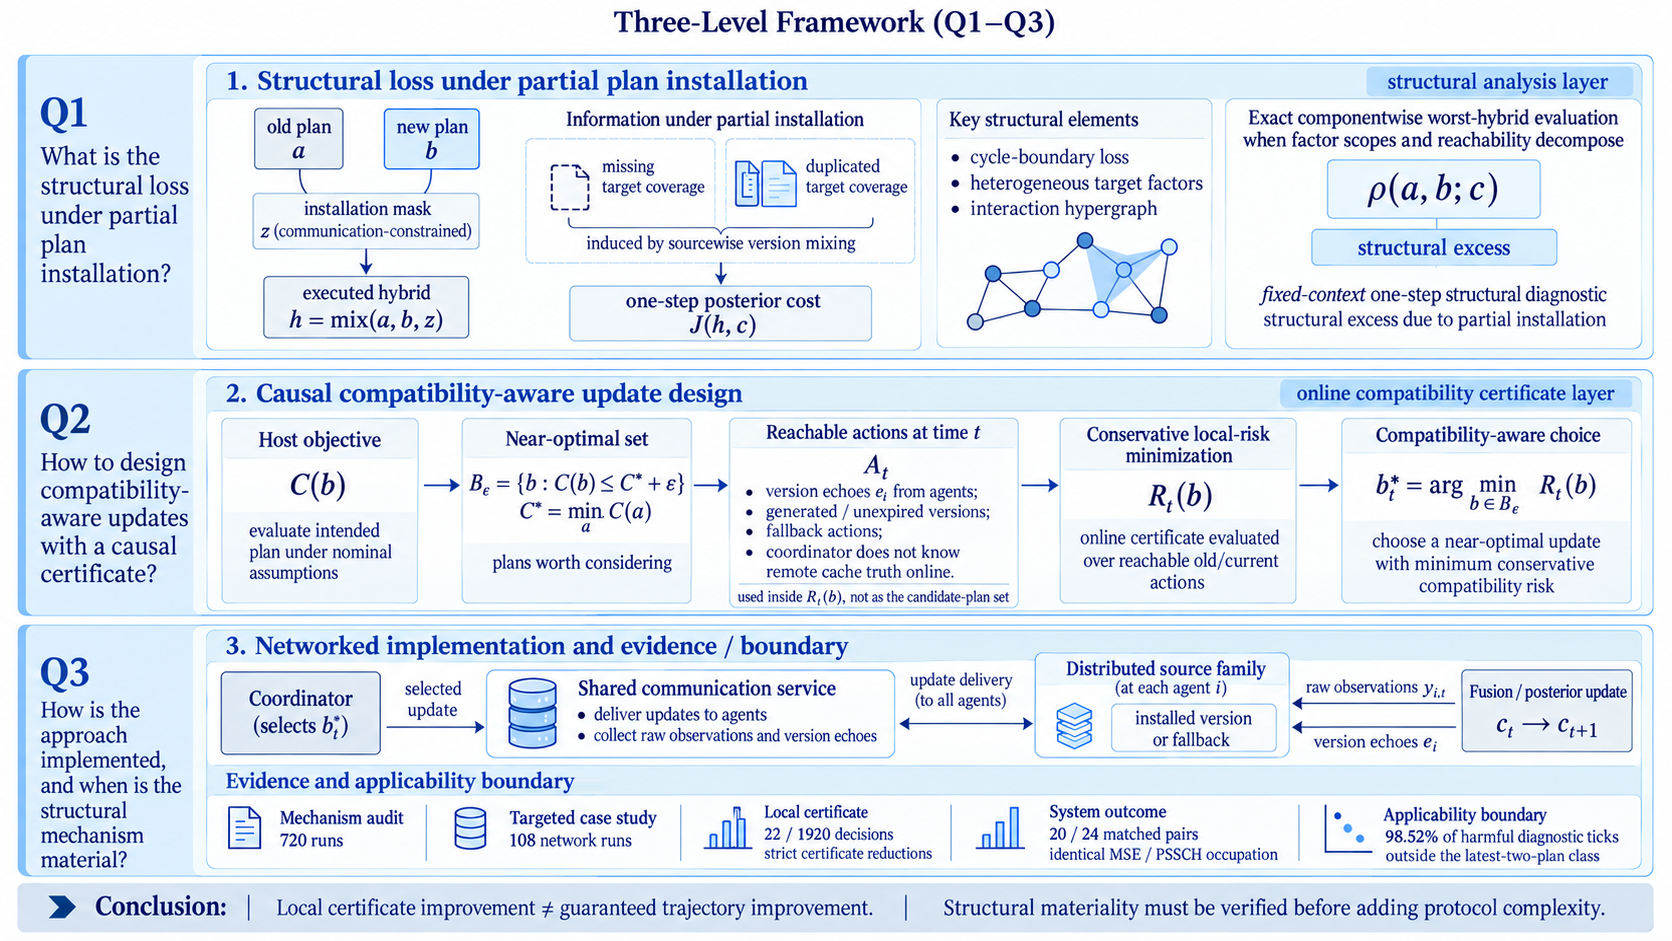
\includegraphics[width=\textwidth]{fig1.png}};
\begin{scope}[x={(framework.south east)},y={(framework.north west)}]
\fill[white] (0.284,0.427) rectangle (0.409,0.474);
\node[text=blue!35!black,font=\fontsize{8}{9}\selectfont] at (0.346,0.451)
  {$C^\star=\min_{\tilde b}C(\tilde b)$};
% Re-typeset only the operational strip, retaining the supplied Q1--Q3 artwork.
\fill[white] (0.127,0.190) rectangle (0.978,0.307);
\node[draw=blue!50,fill=blue!3,rounded corners=2pt,align=center,
 font=\fontsize{8}{9}\selectfont,text=blue!35!black,minimum width=0.24\textwidth,
 minimum height=25pt] (src) at (0.266,0.237)
 {Distributed sources\\Installed plan version\\or fallback};
\node[draw=blue!50,fill=blue!3,rounded corners=2pt,align=center,
 font=\fontsize{8}{9}\selectfont,text=blue!35!black,minimum width=0.21\textwidth,
 minimum height=25pt] (svc) at (0.552,0.237)
 {Shared communication service\\Loss, delay and queues};
\node[draw=blue!50,fill=blue!3,rounded corners=2pt,align=center,
 font=\fontsize{8}{9}\selectfont,text=blue!35!black,minimum width=0.27\textwidth,
 minimum height=25pt] (fusion) at (0.824,0.237)
 {Fusion / coordinator\\Posterior $c_t\!\to\!c_{t+1}$\\Next-round plan $b_{t+1}^{\star}$};
\draw[->,>=stealth,blue!60!black,line width=.7pt] (0.387,0.253)--(0.447,0.253);
\draw[->,>=stealth,blue!60!black,line width=.7pt] (0.658,0.253)--(0.688,0.253);
\draw[->,>=stealth,blue!60!black,line width=.7pt] (0.447,0.219)--(0.387,0.219);
\draw[->,>=stealth,blue!60!black,line width=.7pt] (0.688,0.219)--(0.658,0.219);
\end{scope}
\end{tikzpicture}
